\documentclass{article}

\usepackage[utf8]{inputenc}
\usepackage[T1]{fontenc}
\usepackage[greek,english]{babel}
\usepackage{alphabeta}
\usepackage{amsmath}
\usepackage{amssymb}
\usepackage{graphicx}
\usepackage{subcaption}
\usepackage{epstopdf}
\usepackage[margin=1in, paperwidth=7.5in,paperheight=10.5in]{geometry}
\usepackage{hyperref}
\usepackage{paracol}

\newcommand\course{TΗΛ411}
\newcommand\courseName{Ψηφιακή Επεξεργασία Εικόνας}
\newcommand\semester{Χειμερινό 2021}
\newcommand\assignmentNumber{Assignment 1}
\newcommand\studentName{Μαυρογιώργης Δημήτρης}                           
\newcommand\studentNumber{2016030016}

\title{\underline{\textbf{\assignmentNumber}}} 
\author{\textsc{\textbf{Όνομα:}}  \studentName\\
		\textsc{\textbf{ΑΜ:}}  \studentNumber\\
		\course \ - \courseName\\ 
		\textsc{Πολυτεχνείο Κρήτης}
}
\date{\today}
\begin{document}
	\maketitle

\section*{Introduction}
	Σκοπός της πρώτης εργαστηριακής άσκησης είναι να κάνουμε downsample μια εικόνα χρησιμοποιώντας κάποιες παραμέτρους κλιμάκωσης (1/2, 1/4, 1/8) και έπειτα να κάνουμε upsample το αποτέλεσμα που προέκυψε από το downsample έτσι, ώστε να ανακατασκευάσουμε την αρχική εικόνα. Κατά τη δειγματοληψία εξετάστηκε ο αντύκτυπος της χρήσης ή όχι ενός anti-aliasing φίλτρου, καθώς και κάποιες μέθοδοι interpolation, όπως η nearest-neighbor, bilinear και cubic.
	
\section*{Nearest-Neighbor Interpolation}	
\subsection*{Use of Anti-aliasing Filter}
\begin{figure}[h!]
	\centering
	\begin{subfigure}[t]{0.3\textwidth}
		\centering
		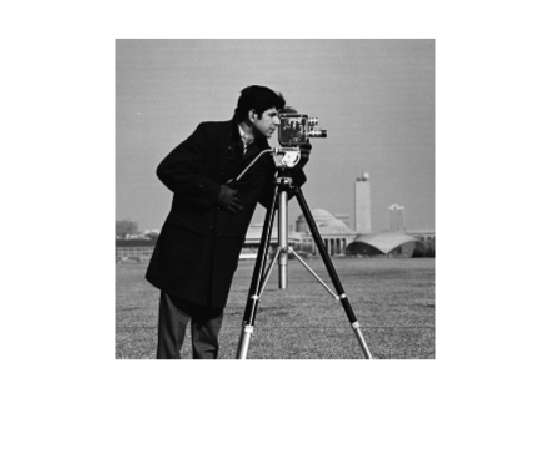
\includegraphics[width=\linewidth]{./output_images/DOWN_anti-alias_nearest_scale_0_500000.png}
		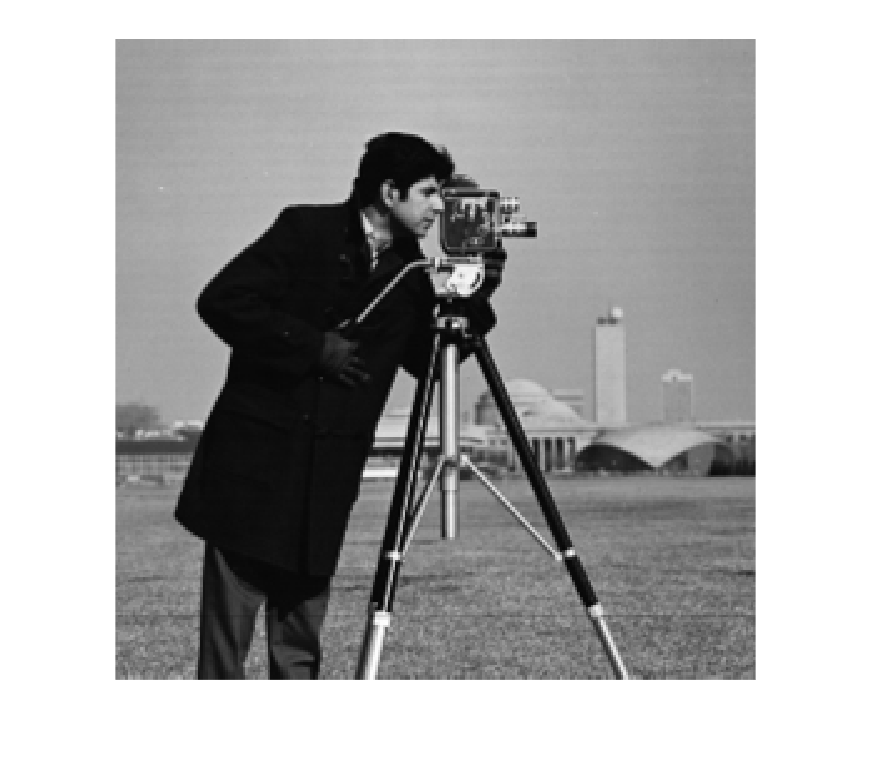
\includegraphics[width=\linewidth]{./output_images/UP_anti-alias_nearest_scale_0_500000.png}
		\caption{Scale 0.5}
	\end{subfigure}%
	~
	\begin{subfigure}[t]{0.3\textwidth}
		\centering
		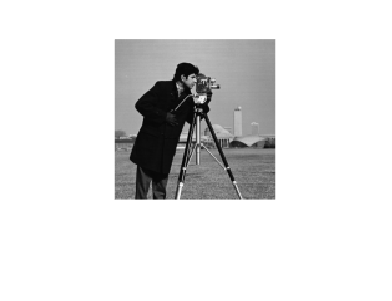
\includegraphics[width=\linewidth]{./output_images/DOWN_anti-alias_nearest_scale_0_250000.png}
		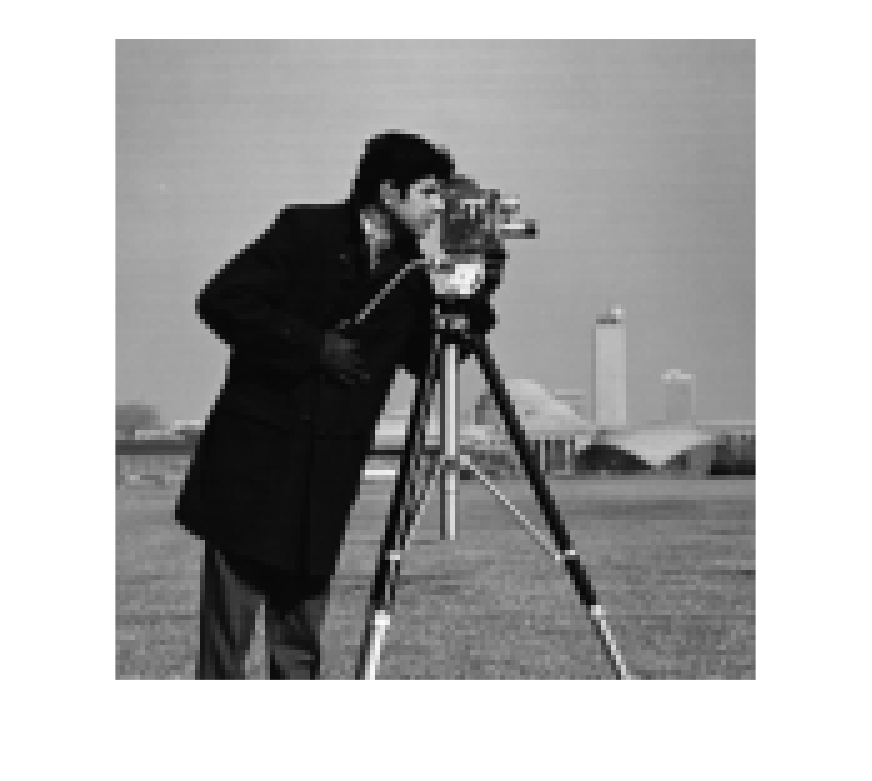
\includegraphics[width=\linewidth]{./output_images/UP_anti-alias_nearest_scale_0_250000.png}
		\caption{Scale 0.25}
	\end{subfigure}
	~
	\begin{subfigure}[t]{0.3\textwidth}
		\centering
		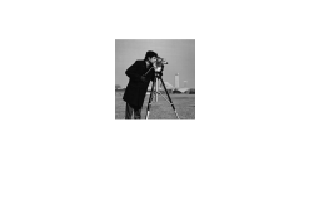
\includegraphics[width=\linewidth]{./output_images/DOWN_anti-alias_nearest_scale_0_125000.png}
		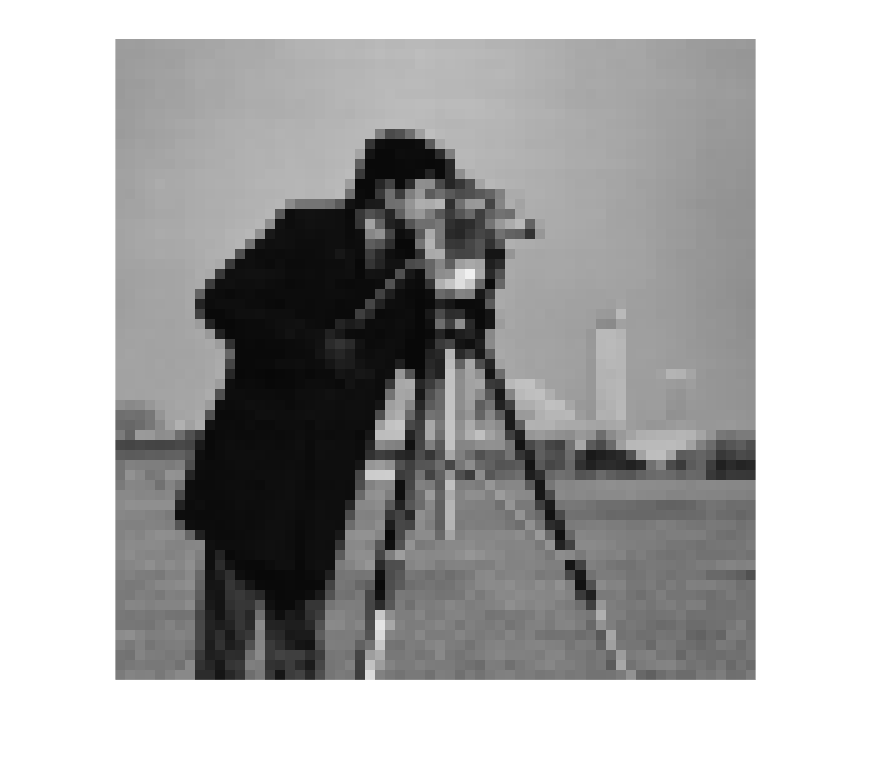
\includegraphics[width=\linewidth]{./output_images/UP_anti-alias_nearest_scale_0_125000.png}
		\caption{Scale 0.125}
	\end{subfigure}
	\caption{Anti-aliasing Filter with nearest-neighbor interpolation}
\end{figure}

\pagebreak

\subsection*{No Use of Anti-aliasing Filter}
\begin{figure}[h!]
	\centering
	\begin{subfigure}[t]{0.3\textwidth}
		\centering
		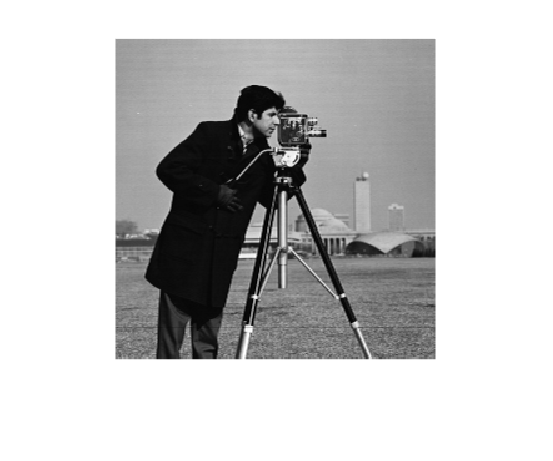
\includegraphics[width=\linewidth]{./output_images/DOWN_no_anti-alias_nearest_scale_0_500000.png}
		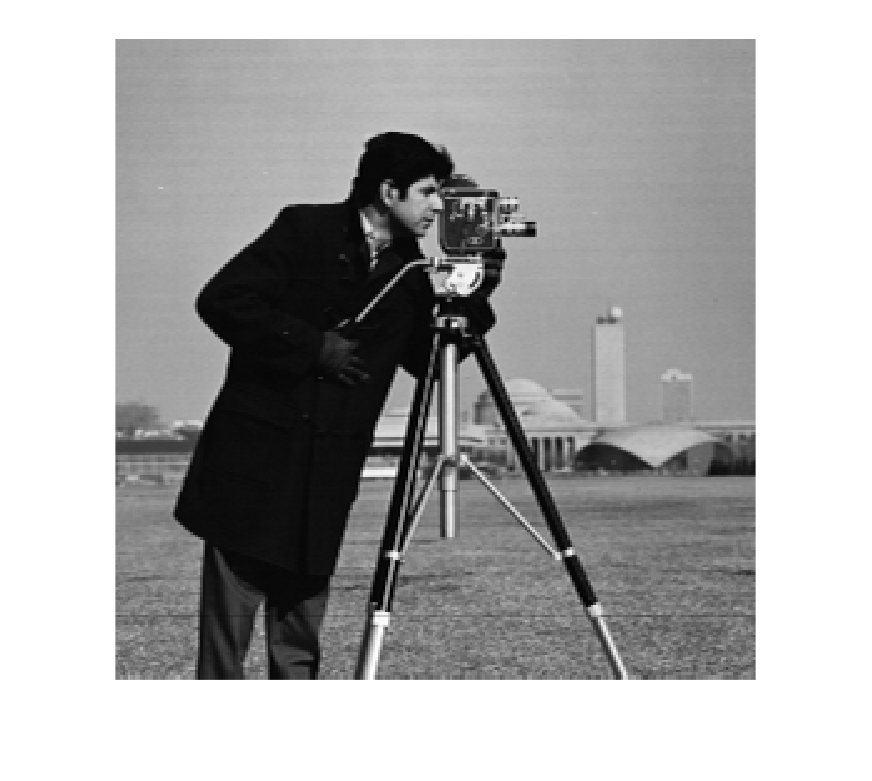
\includegraphics[width=\linewidth]{./output_images/UP_no_anti-alias_nearest_scale_0_500000.png}
		\caption{Scale 0.5}
	\end{subfigure}%
	~
	\begin{subfigure}[t]{0.3\textwidth}
		\centering
		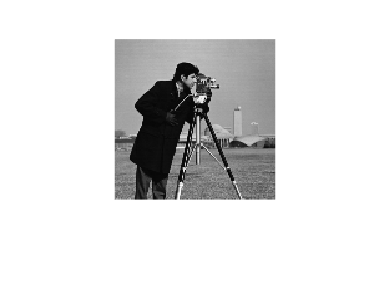
\includegraphics[width=\linewidth]{./output_images/DOWN_no_anti-alias_nearest_scale_0_250000.png}
		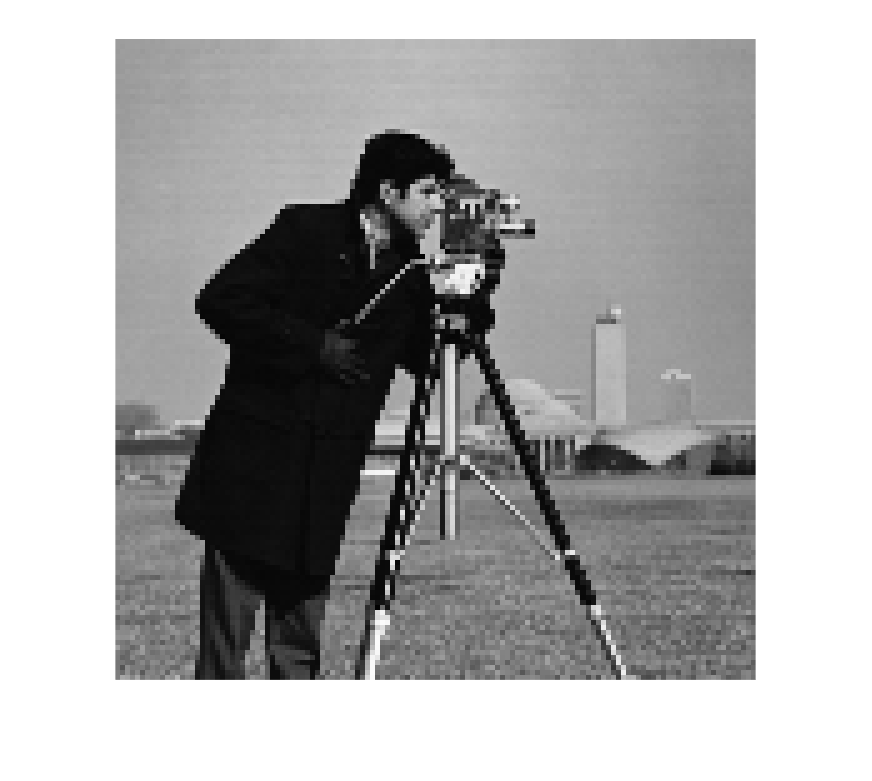
\includegraphics[width=\linewidth]{./output_images/UP_no_anti-alias_nearest_scale_0_250000.png}
		\caption{Scale 0.25}
	\end{subfigure}
	~
	\begin{subfigure}[t]{0.3\textwidth}
		\centering
		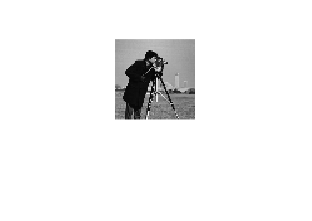
\includegraphics[width=\linewidth]{./output_images/DOWN_no_anti-alias_nearest_scale_0_125000.png}
		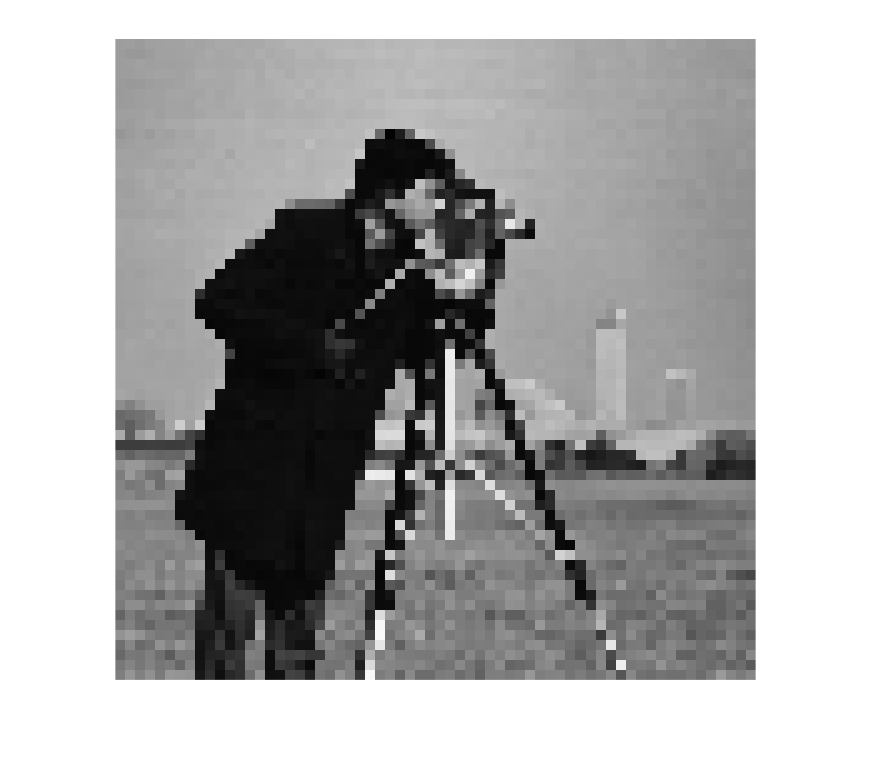
\includegraphics[width=\linewidth]{./output_images/UP_no_anti-alias_nearest_scale_0_125000.png}
		\caption{Scale 0.125}
	\end{subfigure}
	\caption{No Anti-aliasing Filter with nearest-neighbor interpolation}
\end{figure}

\begin{figure}[h!]
	\centering
	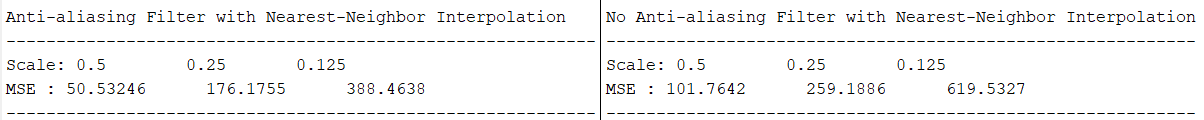
\includegraphics[width=\linewidth]{./output_images/MSE_nearest_neighbor.png}
	\caption{MSE value for nearest-neighbor interpolation}
\end{figure}
	
	\noindent
	Βάση τα παραπάνω αποτελέσματα καταλαβαίνουμε ότι όσο ελαττώνεται η παράμετρος κλιμάκωσης, τόσο μικραίνει η ανάλυση της εικόνας και, επομένως, χάνουμε κάποια πληροφορία κατα την ανάκτηση της εικόνας. Παράλληλα, παρατηρούμε ότι με τη χρήση ενός φίλτρου για anti-aliasing η εικόνα έχει σαφώς πιο βελτιωμένη ανάλυση, γενονός που επαληθεύεται και από το δείκτη MSE, ο οποίος είναι σαφώς πιο μειωμένος στην πρώτη περίπτωση που γίνεται η χρήση του φίλτρου.

\pagebreak

\section*{Bilinear Interpolation}
\subsection*{Use of Anti-aliasing Filter}
\begin{figure}[h!]
	\centering
	\begin{subfigure}[t]{0.3\textwidth}
		\centering
		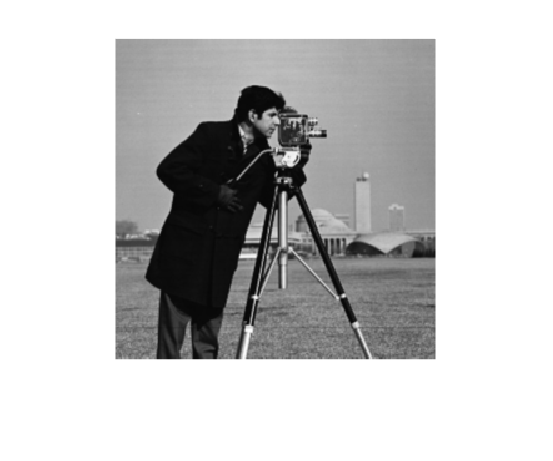
\includegraphics[width=\linewidth]{./output_images/DOWN_anti-alias_bilinear_scale_0_500000.png}
		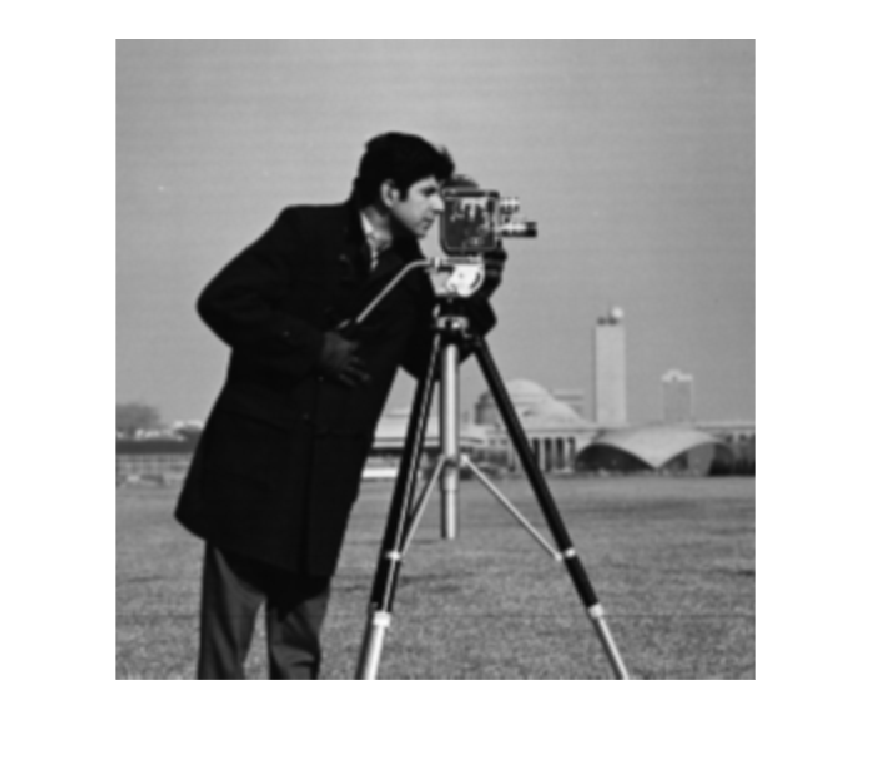
\includegraphics[width=\linewidth]{./output_images/UP_anti-alias_bilinear_scale_0_500000.png}
		\caption{Scale 0.5}
	\end{subfigure}%
	~
	\begin{subfigure}[t]{0.3\textwidth}
		\centering
		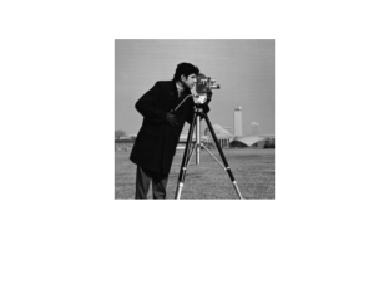
\includegraphics[width=\linewidth]{./output_images/DOWN_anti-alias_bilinear_scale_0_250000.png}
		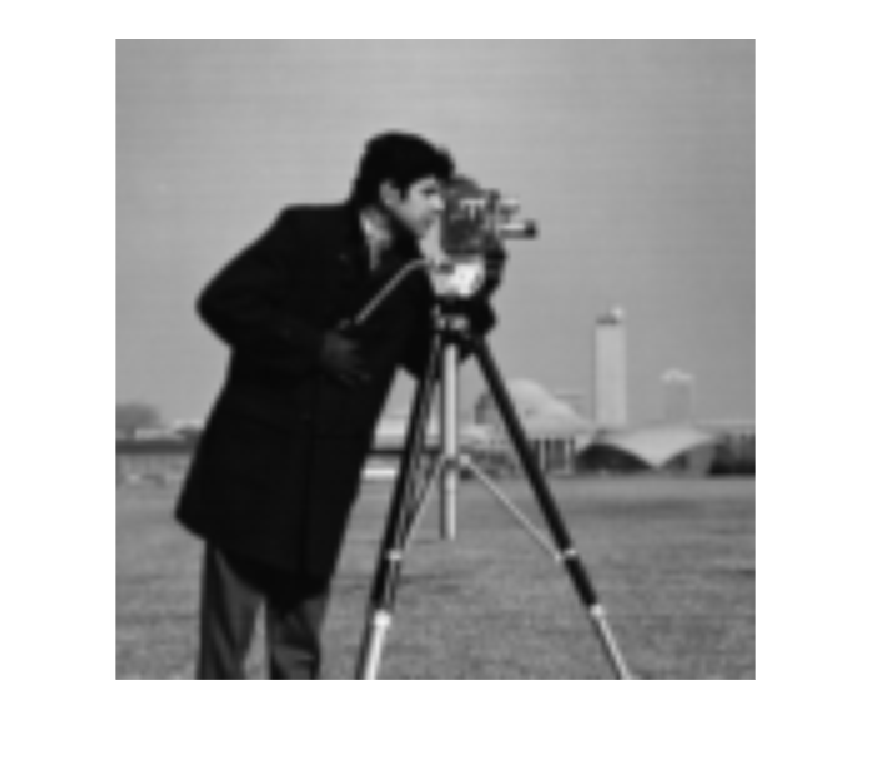
\includegraphics[width=\linewidth]{./output_images/UP_anti-alias_bilinear_scale_0_250000.png}
		\caption{Scale 0.25}
	\end{subfigure}
	~
	\begin{subfigure}[t]{0.3\textwidth}
		\centering
		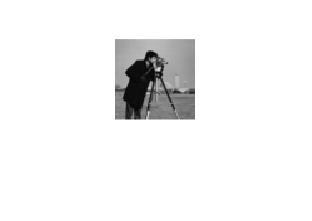
\includegraphics[width=\linewidth]{./output_images/DOWN_anti-alias_bilinear_scale_0_125000.png}
		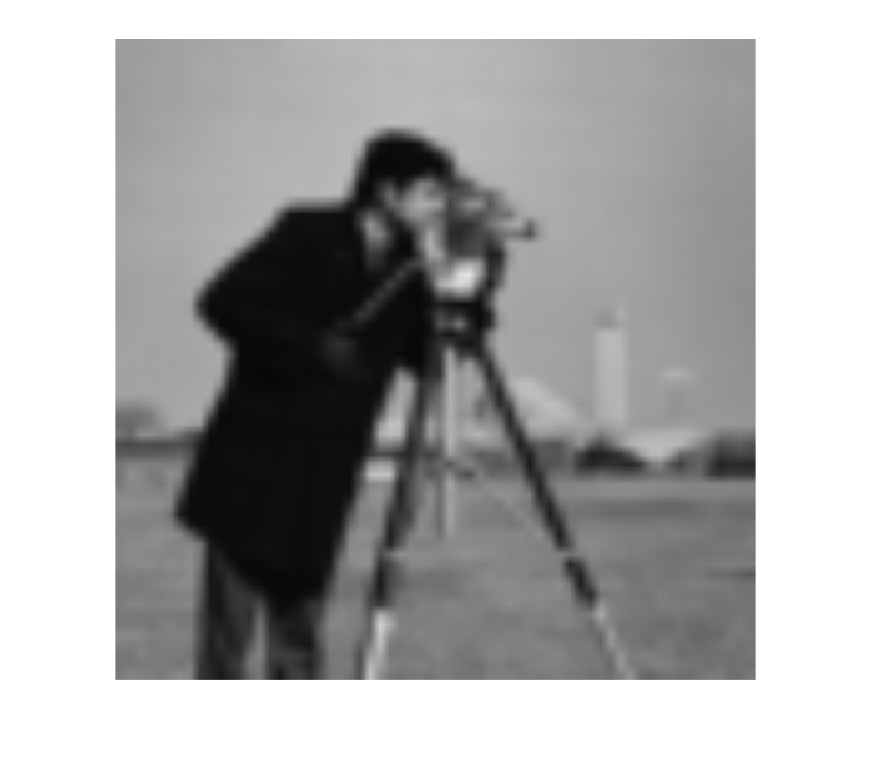
\includegraphics[width=\linewidth]{./output_images/UP_anti-alias_bilinear_scale_0_125000.png}
		\caption{Scale 0.125}
	\end{subfigure}
	\caption{Anti-aliasing Filter with bilinear interpolation}
\end{figure}
	
\subsection*{No Use of Anti-aliasing Filter}
\begin{figure}[h!]
	\centering
	\begin{subfigure}[t]{0.3\textwidth}
		\centering
		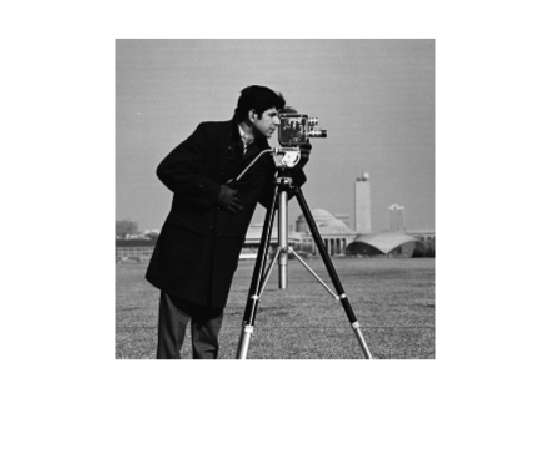
\includegraphics[width=\linewidth]{./output_images/DOWN_no_anti-alias_bilinear_scale_0_500000.png}
		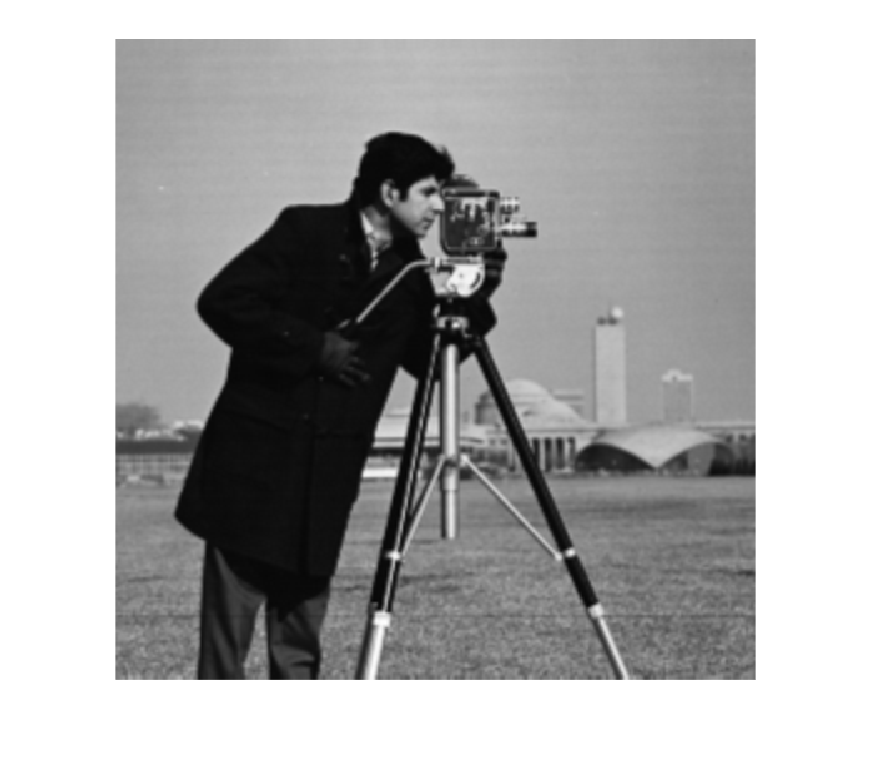
\includegraphics[width=\linewidth]{./output_images/UP_no_anti-alias_bilinear_scale_0_500000.png}
		\caption{Scale 0.5}
	\end{subfigure}%
	~
	\begin{subfigure}[t]{0.3\textwidth}
		\centering
		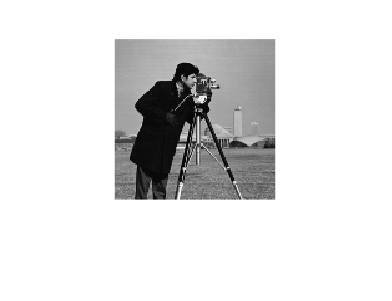
\includegraphics[width=\linewidth]{./output_images/DOWN_no_anti-alias_bilinear_scale_0_250000.png}
		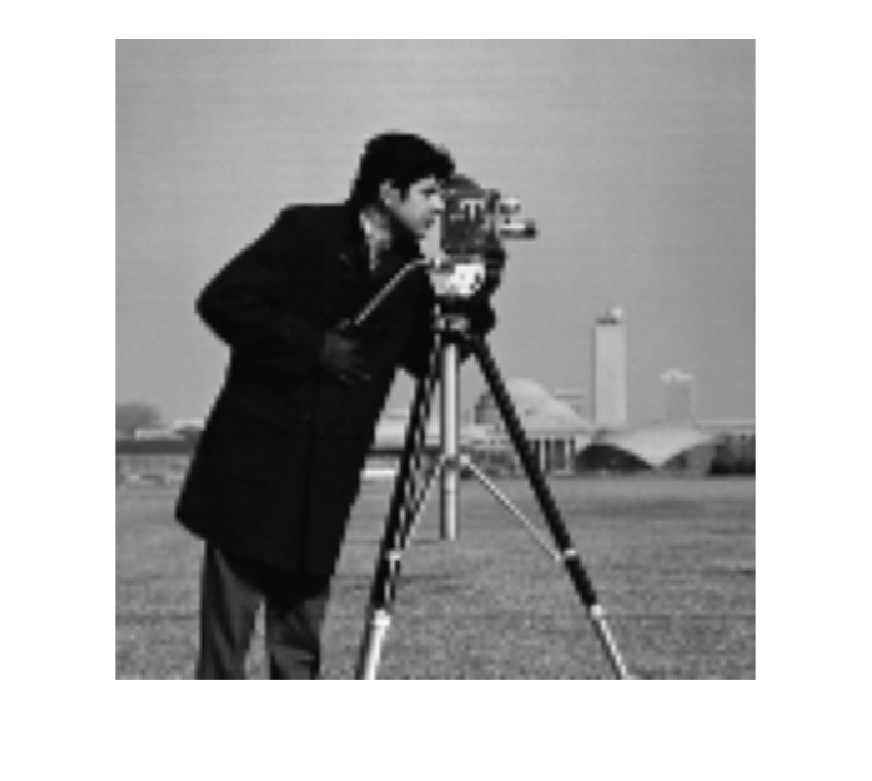
\includegraphics[width=\linewidth]{./output_images/UP_no_anti-alias_bilinear_scale_0_250000.png}
		\caption{Scale 0.25}
	\end{subfigure}
	~
	\begin{subfigure}[t]{0.3\textwidth}
		\centering
		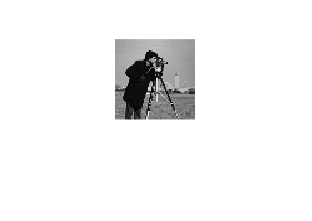
\includegraphics[width=\linewidth]{./output_images/DOWN_no_anti-alias_bilinear_scale_0_125000.png}
		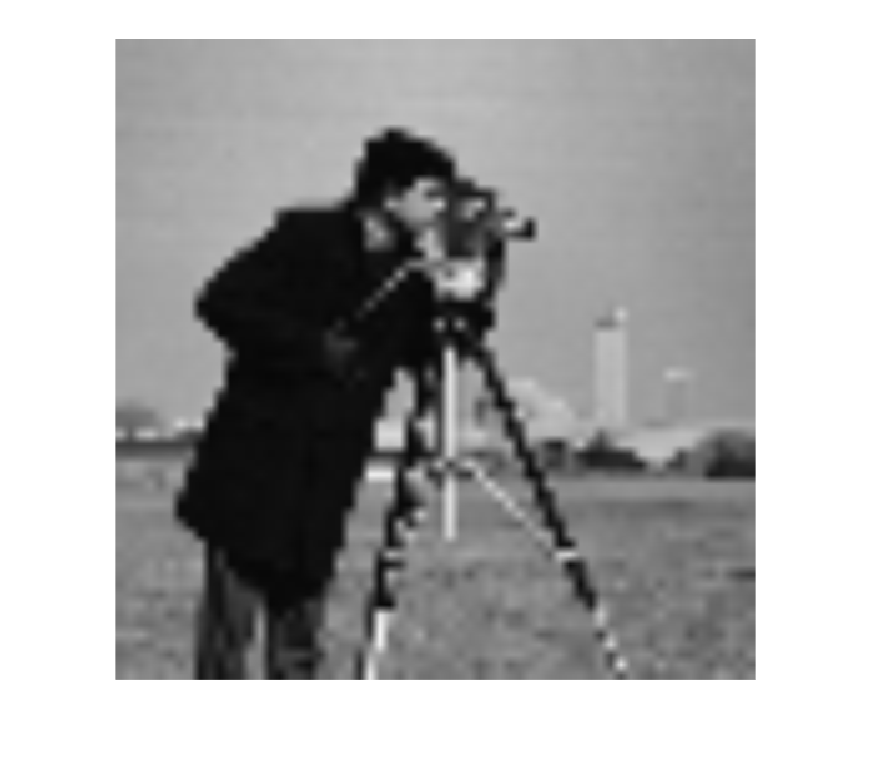
\includegraphics[width=\linewidth]{./output_images/UP_no_anti-alias_bilinear_scale_0_125000.png}
		\caption{Scale 0.125}
	\end{subfigure}
	\caption{No Anti-aliasing Filter with bilinear interpolation}
\end{figure}

\pagebreak

\begin{figure}[h!]
	\centering
	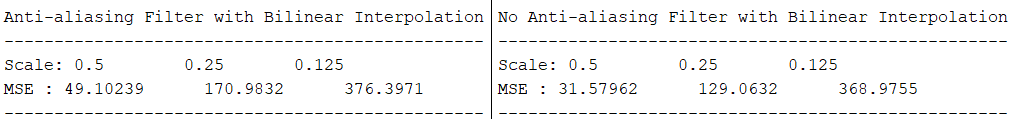
\includegraphics[width=\linewidth]{./output_images/MSE_bilinear.png}
	\caption{MSE value for bilinear interpolation}
\end{figure}

	\noindent
	Και σε αυτή την περίπτωση παρατηρούμε ότι όσο ελαττώνεται η παράμετρος κλιμάκωσης, τόσο μικραίνει η ανάλυση της εικόνας και χάνουμε κάποια πληροφορία από την αρχική εικόνα. Μια αρκετά εμφανής διαφορά είναι ότι με τη χρήση του φίλτρου anti-aliasing η εικόνα γίνεται πιο θολή σε σχέση με την αρχική και με την περίπτωση μη χρήσης φίλτρου. Όσον αφορά το MSE βλέπουμε ότι στην περίπτωση που δε χρησιμοποιούμε το φίλτρο η τιμή είναι ελαφρώς μικρότερη, γεγονός που δικαιολογεί τη χειρότερη ανάλυση και ευκρίνεια στην περίπτωσης χρήσης του φίλτρου.
\section*{Cubic Interpolation}
\subsection*{Use of Anti-Aliasing Filter}
\begin{figure}[h!]
	\centering
	\begin{subfigure}[t]{0.3\textwidth}
		\centering
		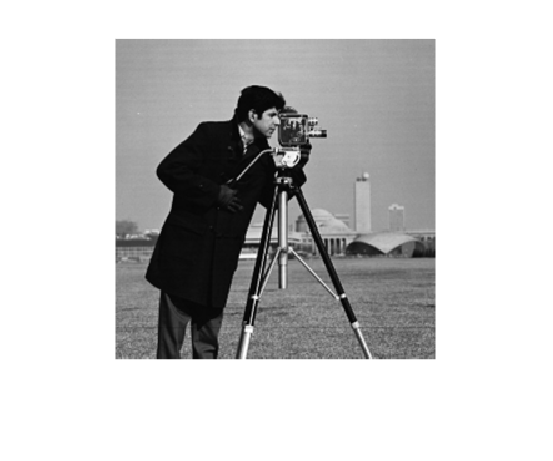
\includegraphics[width=\linewidth]{./output_images/DOWN_anti-alias_cubic_scale_0_500000.png}
		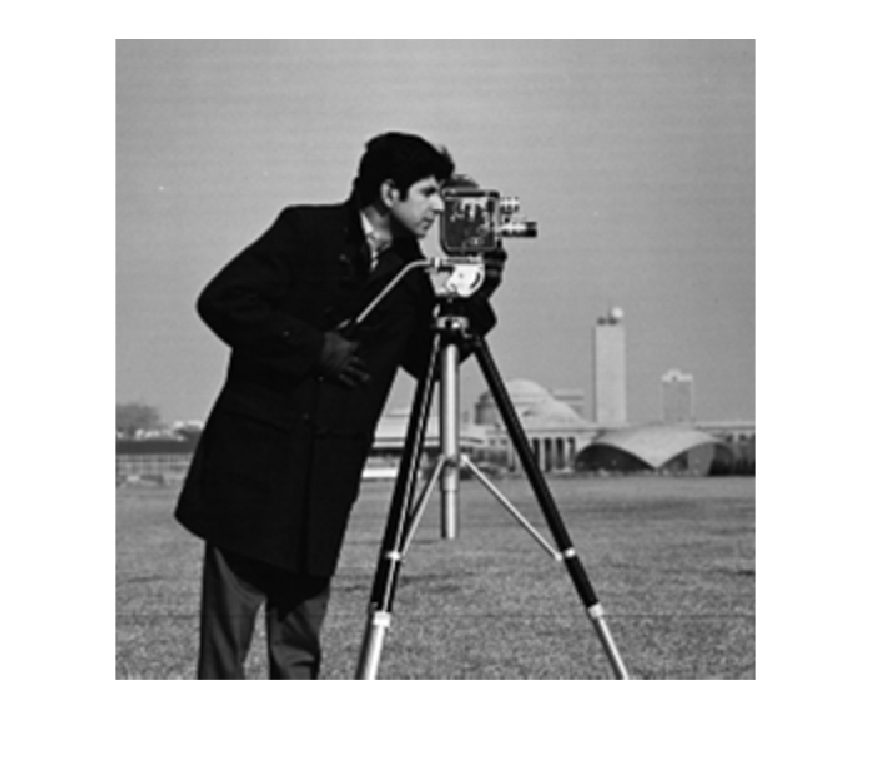
\includegraphics[width=\linewidth]{./output_images/UP_anti-alias_cubic_scale_0_500000.png}
		\caption{Scale 0.5}
	\end{subfigure}%
	~
	\begin{subfigure}[t]{0.3\textwidth}
		\centering
		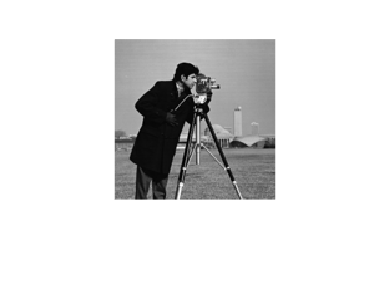
\includegraphics[width=\linewidth]{./output_images/DOWN_anti-alias_cubic_scale_0_250000.png}
		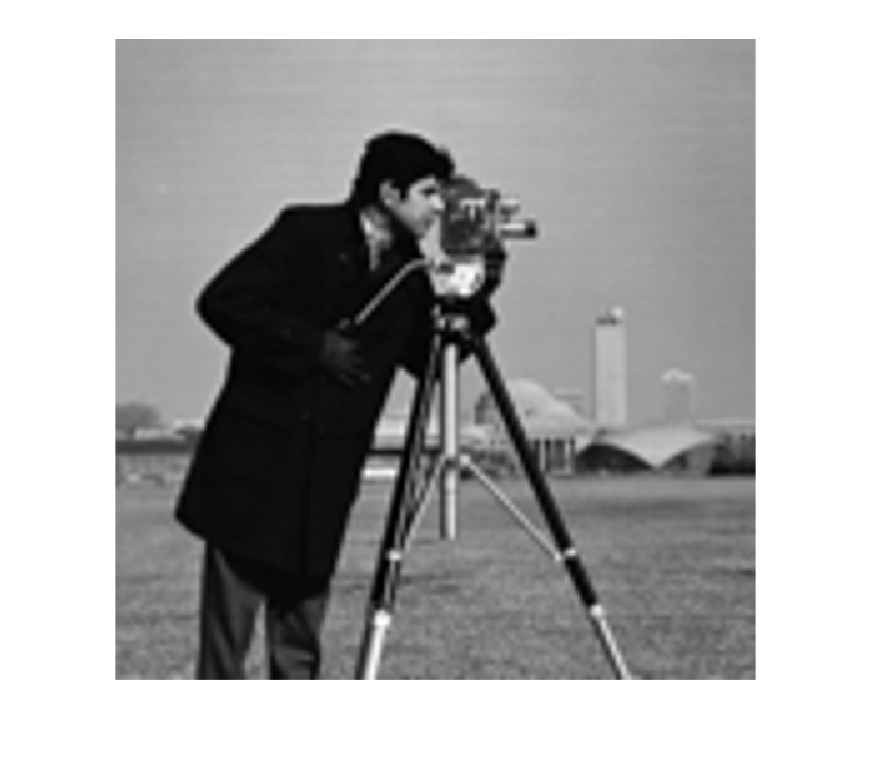
\includegraphics[width=\linewidth]{./output_images/UP_anti-alias_cubic_scale_0_250000.png}
		\caption{Scale 0.25}
	\end{subfigure}
	~
	\begin{subfigure}[t]{0.3\textwidth}
		\centering
		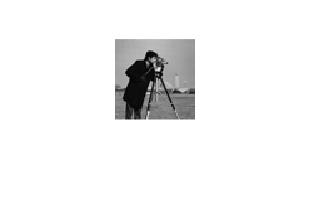
\includegraphics[width=\linewidth]{./output_images/DOWN_anti-alias_cubic_scale_0_125000.png}
		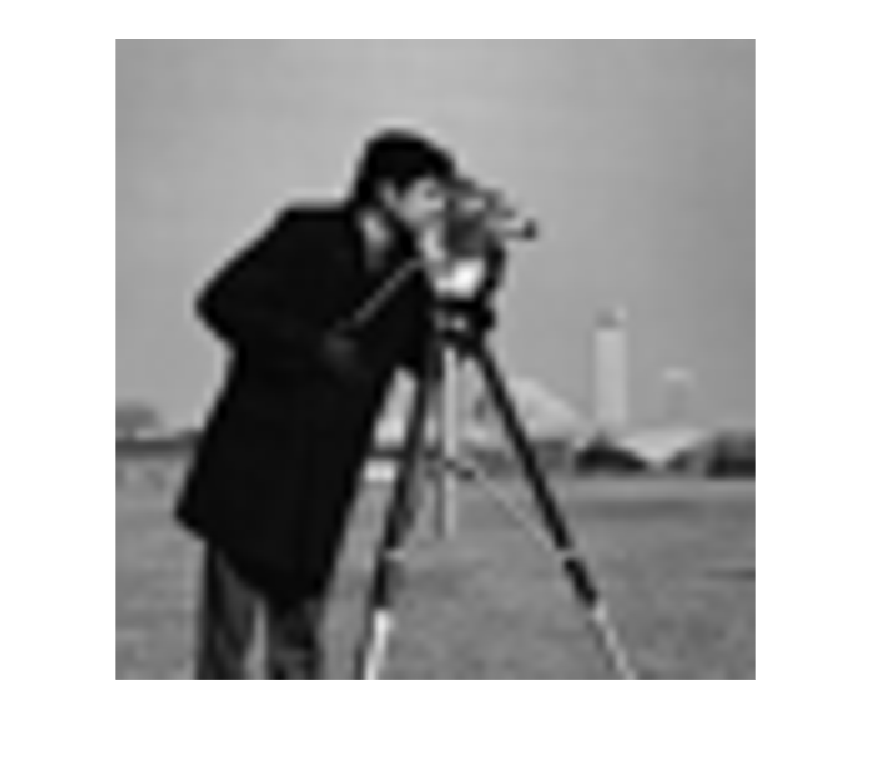
\includegraphics[width=\linewidth]{./output_images/UP_anti-alias_cubic_scale_0_125000.png}
		\caption{Scale 0.125}
	\end{subfigure}
	\caption{Anti-aliasing Filter with cubic interpolation}
\end{figure}

\pagebreak

\subsection*{No Use of Anti-Aliasing Filter}
\begin{figure}[h!]
	\centering
	\begin{subfigure}[t]{0.3\textwidth}
		\centering
		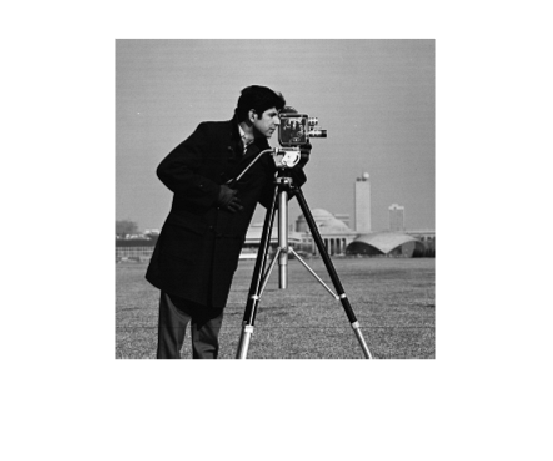
\includegraphics[width=\linewidth]{./output_images/DOWN_no_anti-alias_cubic_scale_0_500000.png}
		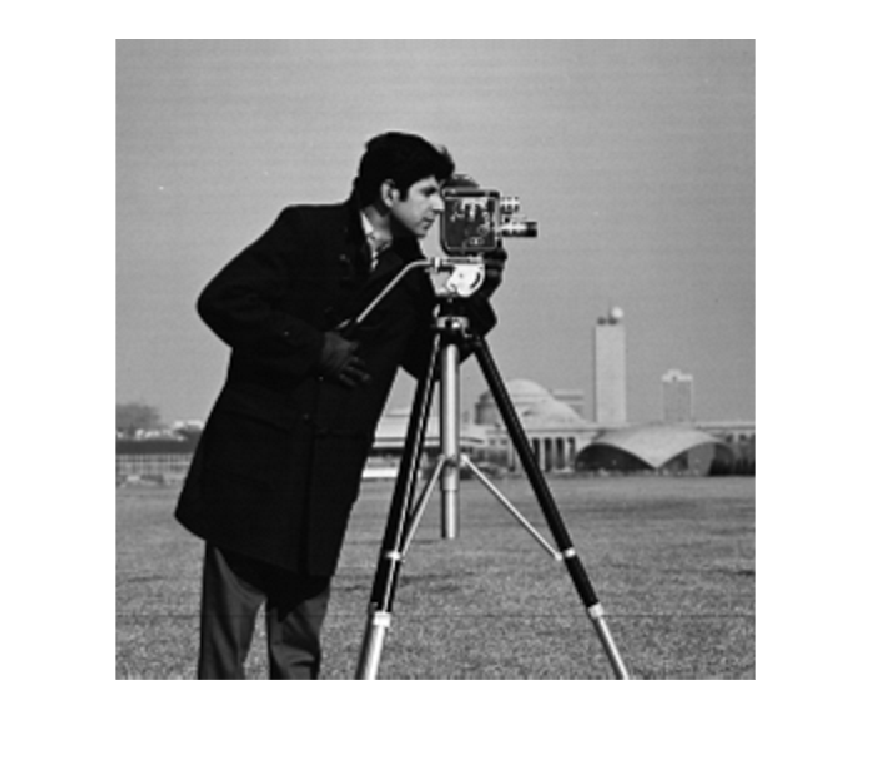
\includegraphics[width=\linewidth]{./output_images/UP_no_anti-alias_cubic_scale_0_500000.png}
		\caption{Scale 0.5}
	\end{subfigure}%
	~
	\begin{subfigure}[t]{0.3\textwidth}
		\centering
		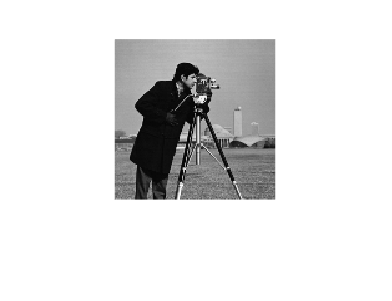
\includegraphics[width=\linewidth]{./output_images/DOWN_no_anti-alias_cubic_scale_0_250000.png}
		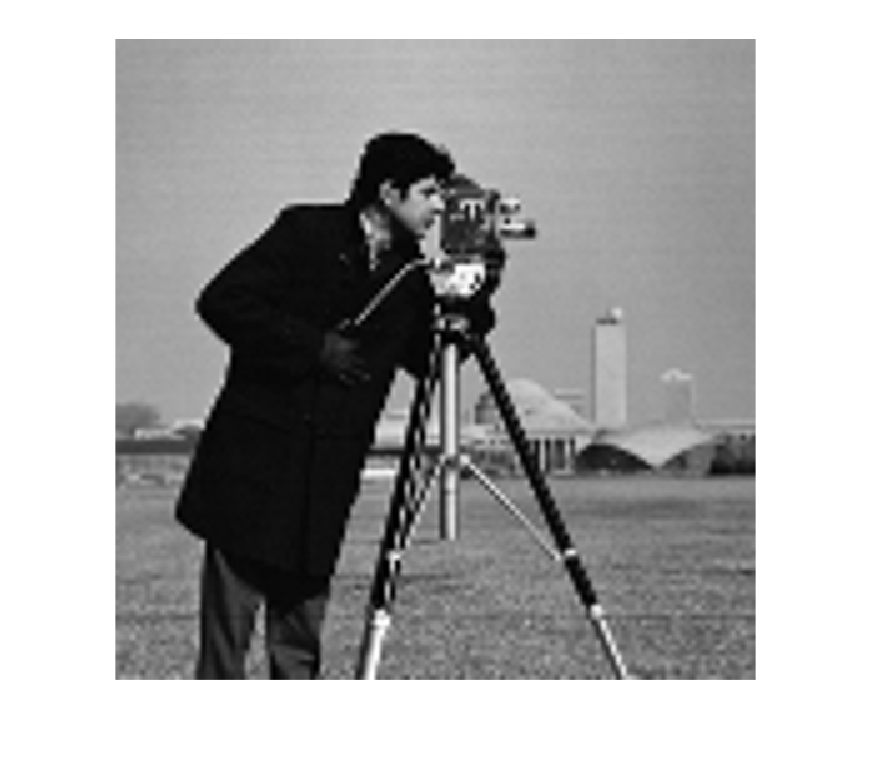
\includegraphics[width=\linewidth]{./output_images/UP_no_anti-alias_cubic_scale_0_250000.png}
		\caption{Scale 0.25}
	\end{subfigure}
	~
	\begin{subfigure}[t]{0.3\textwidth}
		\centering
		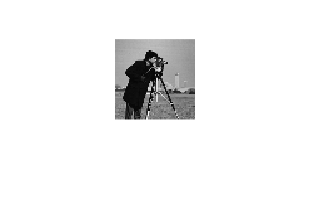
\includegraphics[width=\linewidth]{./output_images/DOWN_no_anti-alias_cubic_scale_0_125000.png}
		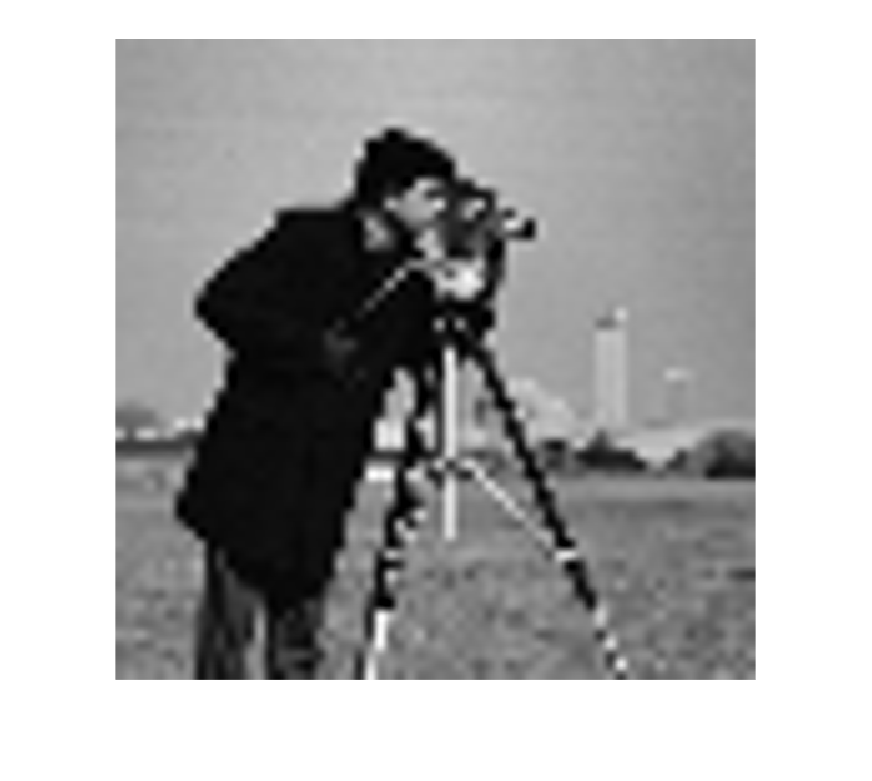
\includegraphics[width=\linewidth]{./output_images/UP_no_anti-alias_cubic_scale_0_125000.png}
		\caption{Scale 0.125}
	\end{subfigure}
	\caption{No Anti-aliasing Filter with cubic interpolation}
\end{figure}

\begin{figure}[h!]
	\centering
	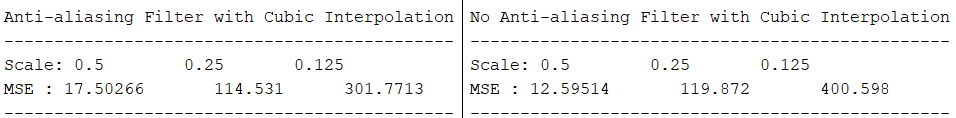
\includegraphics[width=\linewidth]{./output_images/MSE_cubic.png}
	\caption{MSE value for cubic interpolation}
\end{figure}
	\noindent
	Σε αυτή την περίπτωση, παρατηρούμε ότι, καθώς μειώνεται η παράμετρος κλιμάκωσης, έχουμε ελάττωση της ανάλυσης. Επιπλέον, βλέπουμε ότι με τη χρήση φίλτρου κατα τη ανάκτηση της εικόνας, περιορίζουμε την μεγάλη απώλεια στην ανάλυσή της. Όσον αφορά το δείκτη MSE, βλέπουμε ότι η χρήση φίλτρου χειροτερεύει ελαφρώς το δείκτη MSE στην περίπτωση που το scale είναι 1/2, ενώ στις άλλες δύο περιπτώσεις υπάρχει αρκετή βελτίωση με τη χρήση του. \\
	\\
	\noindent
	Τέλος, συγκρίνοντας όλα τα παραπάνω αποτελέσματα παρατηρούμε ότι η καλύτερη μέθοδος ανάκτησης μίας εικόνας, όταν έχουμε χρήση του φίλτρου anti-aliasing, είναι η cubic interpolation. Αντίθετα, όταν δε χρησιμοποιούμε κάποιο φίλτρο, η καλύτερη μέθοδος είναι η bilinear για scale 1/8, ενώ για τις άλλες δύο περιπτώσεις scale η καλύτερη είναι η cubic. Tα αποτελέσματα αυτά επαληθεύονται και με βάση το δείκτη MSE σε κάθε περίπτωση. 
\end{document}
